\documentclass[a4paper,12pt]{article}
%%%%%%%%%%%%%%%%%%%%%%%%%%%%%%%%%%%%%%%%%%%%%%%%%%%%%%%%%%%%%%%%%%%%%%%%%%%%%%%%%%%%%%%%%%%%%%%%%%%%%%%%%%%%%%%%%%%%%%%%%%%%%%%%%%%%%%%%%%%%%%%%%%%%%%%%%%%%%%%%%%%%%%%%%%%%%%%%%%%%%%%%%%%%%%%%%%%%%%%%%%%%%%%%%%%%%%%%%%%%%%%%%%%%%%%%%%%%%%%%%%%%%%%%%%%%
\usepackage{eurosym}
\usepackage{vmargin}
\usepackage{amsmath}
\usepackage{framed}
\usepackage{graphics}
\usepackage{epsfig}
\usepackage{subfigure}
\usepackage{fancyhdr}

\setcounter{MaxMatrixCols}{10}
%TCIDATA{OutputFilter=LATEX.DLL}
%TCIDATA{Version=5.00.0.2570}
%TCIDATA{<META NAME="SaveForMode" CONTENT="1">}
%TCIDATA{LastRevised=Wednesday, February 23, 2011 13:24:34}
%TCIDATA{<META NAME="GraphicsSave" CONTENT="32">}
%TCIDATA{Language=American English}

\pagestyle{fancy}
\setmarginsrb{20mm}{0mm}{20mm}{25mm}{12mm}{11mm}{0mm}{11mm}
\lhead{MS4222} \rhead{Mr. Kevin O'Brien}
\chead{Continuous Uniform Distribution}
%\input{tcilatex}

\begin{document}


\section*{Continuous Uniform Distribution}
%=====================================================================%
%\textbf{Continuous Uniform Distribution} 
\begin{itemize}
	\item  
	The Uniform family of distributions model (some) continuous random variables and (some) discrete random variables. The values of a uniform random variable are uniformly distributed over an interval. 

\item The continuous uniform distribution is very simple to understand and implement, and is commonly used in computer applications. This probability distribution is particularly useful in computer simulations. It is very simple to understand, and is a good starting place for learning about continuous probability distributions.
\textit{(It is also known as the `Rectangle Distribution' for obvious reasons)}.
\item We specify the word ``continuous" so as to distinguish it from it's discrete equivalent: the discrete uniform distribution.\\ \textit{Remark; the dice distribution is a discrete uniform distribution with lower and upper limits 1 and 6 respectively.}
	\item 
For example, if buses arrive at a given bus stop every 8 minutes, and you arrive at the bus stop at a random time, the time you wait for the 
next bus to arrive could be described by a uniform distribution over the interval from 0 to 8.
\end{itemize}


\begin{figure}[h!]
	\centering
	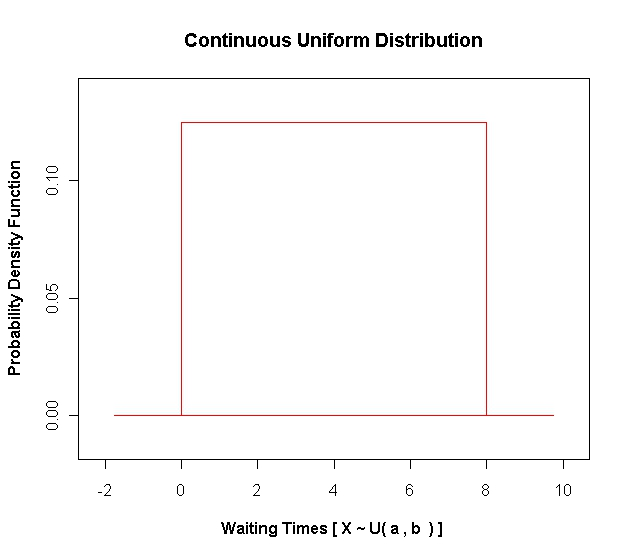
\includegraphics[width=0.5\linewidth]{images/6AUniform}
	\caption{}
	\label{fig:6AUniform}
\end{figure}


\subsection*{Parameters of the Uniform Distribution}
\begin{itemize}

\item The uniform distribution is characterized by the two values, the \textbf{minimum} ($a$) and the \textbf{maximum} ($b$). Any value between $a$ and $b$ has an equal likelihood of occuring.
\item When $X$ is a uniformly distributed random variables, we would describe it mathematically as follows:
\[ X \sim U(a,b). \]

\item It is not possible to have an outcome that is lower than $a$ or larger than $b$.

\[ P(X < a) = P(X > b) = 0\] 

\item In the absence of the specified upper and lower limits, the default values of 0 and 1 would be used.



% \item The expected value E(x) is given by (i.e. the average of the maximum and minimum)
% \[ E(X) = {a+b \over 2}\]
% \item The variance of the continuous uniform distribution is
% \[ V(X) = {(b-a)^2\over12}\]
\end{itemize}


% http://www.saylor.org/site/wp-content/uploads/2011/06/MA121-3.2.2.pdf

\begin{framed}
\noindent A random variable X is called a continuous uniform random variable over the interval $(a,b)$ if it's probability density function is given by
\[ f_{X}(x) = { 1 \over b-a} \hspace{1cm} \mbox{ when } a \leq x \leq b \mbox{     (otherwise } f_X(x) = 0 ) \]
The corresponding cumulative density function is
\[ F_x(x) = { x-a \over b-a} \hspace{1cm} \mbox{ when } a \leq x \leq b\]
\end{framed}



%---------------------------------------------------------------------------%
\subsection*{Sample Space}
\noindent Suppose that a continuous uniform distribution is characterized by the following parameter values:
\begin{itemize}
\item The lower limit $a = 3$. % (or with \texttt{R}: \texttt{\textbf{min}} )

\item The upper limit $b = 6$. % (or with \texttt{R}: \texttt{\textbf{max}} )
\item We denote $X$ as $X \sim U(3,6)$
\end{itemize}



% \begin{itemize}
%\item[a:] The lowest possible value of $X$ (i.e. the minimum)
%\item[b:] The highest possible value of $X$ (i.e. the maximum)
% \end{itemize} 
%------------------------------------------------------------------------%
\begin{itemize}
\item  The following values are possible outcomes: $3.14, \;3.78,\; 4.66,\; 5.8,\;5.9999.$ \smallskip
\item  The probability of being exactly equal to $3$ or $6$ can be assumed to be zero. \smallskip
\item  The following outcomes are not possible, either because they are too high or too low.
$1.67,\;2,\;67,\;7.14,\; 8.78.$
\end{itemize}
%========================================================================%



\subsection*{Interval Probability}

\begin{itemize}
	\item We wish to compute the probability of an outcome being within a range of values.
	\item We shall call this lower bound of this range $L$ and the upper bound $ U$.
	\item Necessarily $L$ and $U$ must be possible outcomes.
	\item The probability of $X$ being between $L$ and $U$ is denoted $P( L \leq X \leq U )$.
	
	\[
	P( L \leq X \leq U ) = { U - L \over b - a}
	\]
	\item \textit{(This equation is based on a definite integral)}.

\end{itemize}


%============================================================ %

\subsection*{Reminder}

\begin{itemize}
\item " $\leq$" is less than or equal to
	
\item " $\geq$" is greater than or equal to
\end{itemize}

The mathematical statement
\[L \leq X \leq U\]

simply states that X is between L and U inclusively. $X$ could be exactly L or U also, although the probability of this is extremely low.


\begin{itemize}
	
	\item For any value ``c" between the minimum value $a$ and the maximum
	value $b$, we can express $P(X \leq c)$ as
	\[P(X \leq c) = {c-a \over b-a}.\]
	Here $c$ is the upper bound while $a$ is the lower bound.
	\item Similarly $P(X \geq c)$ \[P(X \geq c) = {b-c \over b-a}.\]
	Here $b$ is the upper bound while $c$ is the lower bound.
\end{itemize}



% http://www.saylor.org/site/wp-content/uploads/2011/06/MA121-3.2.2.pdf


%%\subsubsection{Generating Random Values}
%%The most common use of the uniform distribution is the generation of uniformly distributed random variables. 
%%
%%
%%The relevant command is \texttt{\textbf{runif()}}. 
%%Functions that can be used to manage precision are useful when generating random values.
%%
%%\begin{verbatim}
%%> runif(10)
%%[1] 0.2558100 0.8738507 0.4521578 0.7868320 0.2310644 0.5265236
%%[7] 0.9041761 0.3948904 0.1928505 0.5793142
%%> runif(10,min=1,max=7)
%%[1] 2.822485 4.603547 5.794749 3.766398 2.016349 2.116504 5.863682
%%[8] 3.911420 3.434373 6.986899
%%>
%%> Another Way of Simulating Dice Rolls
%%> floor(runif(10,min=1,max=7))
%%[1] 1 5 1 6 6 2 1 2 6 3
%%\end{verbatim}





\subsection*{Uniform Distribution : Expected Value and Variance}
The expected Value of a uniformly distributed random variable $X$, specifed with maximum value $b$ and minimum value $a$, i.e.
\[ X \sim U(a,b) \] is computed using the following formula
\[ E(X) = \frac{a+b}{2}. \]




%R Code for Graphics
%
%y=c(20,20)
%x=c(20,100)
%
%plot(x,y,xlim=c(0,120),ylim=c(0,30),pch=13,col='white',axes=FALSE)
%segments(20,20,100,20,col= 'red')
%segments(0,0,120,0)
%
%segments(20,0,20,20,col='red')
%segments(100,0,100,20,col='red')
%
%segments(0,0,0,40)



\noindent The variance of the continuous uniform distribution, denoted $\textrm{Var}(X)$, is computed using the following formula
%% \vspace{0.1cm}
\[
\textrm{Var}(X) = {(b - a)^2 \over 12}
\]
%% \vspace{0.1cm}
Suppose $X \sim U(3,6)$ then
\[
\textrm{Var}(X) = {{(6 - 3)^2 \over 12} =  {3^2 \over 12} = {9 \over 12} = 0.75}
\]








% http://www.saylor.org/site/wp-content/uploads/2011/06/MA121-3.2.2.pdf





%%\subsubsection{Generating Random Values}
%%The most common use of the uniform distribution is the generation of uniformly distributed random variables. 
%%
%%
%%The relevant command is \texttt{\textbf{runif()}}. 
%%Functions that can be used to manage precision are useful when generating random values.
%%
%%\begin{verbatim}
%%> runif(10)
%%[1] 0.2558100 0.8738507 0.4521578 0.7868320 0.2310644 0.5265236
%%[7] 0.9041761 0.3948904 0.1928505 0.5793142
%%> runif(10,min=1,max=7)
%%[1] 2.822485 4.603547 5.794749 3.766398 2.016349 2.116504 5.863682
%%[8] 3.911420 3.434373 6.986899
%%>
%%> Another Way of Simulating Dice Rolls
%%> floor(runif(10,min=1,max=7))
%%[1] 1 5 1 6 6 2 1 2 6 3
%%\end{verbatim}
%%



\end{document}


